\documentclass[oneside,12pt,letterpaper]{article}

% Imports and Definitions
%% Packages
\usepackage{amsmath}
\usepackage{amsfonts}
\usepackage{amssymb}
\usepackage{amsthm}
\usepackage{arydshln}
\usepackage{color}
\usepackage{extramarks}
\usepackage{fancyhdr}
\usepackage{float}
\usepackage[margin=1in]{geometry}
\usepackage{graphicx}
\usepackage{listings}
\usepackage{multicol}
\usepackage{setspace}
\usepackage{subcaption}
\usepackage{textcomp}
\usepackage{url}
\usepackage{xspace}
\usepackage{mathtools}

%% Commands
%%% Metadata
\newcommand{\metaTitle}{Comprehensive Exam}
\newcommand{\metaDueDate}{November 24, 2020}
\newcommand{\metaDueTime}{04:00 PM}
\newcommand{\metaSchool}{IUPUI}
\newcommand{\metaClass}{STAT 52400}
\newcommand{\metaDepartment}{Statistics Department}
\newcommand{\metaAuthorName}{Ross Grinvalds}

%%% Aliases
\newcommand{\Bias}{\mathrm{Bias}}
\newcommand{\Cov}{\mathrm{Cov}}
\newcommand{\dd}[1]{\frac{\mathrm{d}}{\mathrm{d}x} (#1)}
\newcommand{\dx}{\mathrm{d}x}
\newcommand{\E}{\mathrm{E}}
\newcommand{\m}[1]{\begin{bmatrix*}[r]#1\end{bmatrix*}}
\newcommand{\md}[1]{\begin{vmatrix*}#1\end{vmatrix*}}
\newcommand{\mf}[1]{\mathrm{\bf{#1}}}
\newcommand{\p}[1]{\begin{pmatrix}#1\end{pmatrix}} 
\newcommand{\pdd}[2]{\frac{\partial}{\partial #1} (#2)}
\newcommand{\solution}{\textbf{\large Solution}}
\newcommand{\T}{\intercal}
\newcommand{\Var}{\mathrm{Var}}

%%% Math Functions
\makeatletter
\newsavebox{\mybox}\newsavebox{\mysim}
\newcommand{\distras}[1]{%
  \savebox{\mybox}{\hbox{\kern3pt$\scriptstyle#1$\kern3pt}}%
  \savebox{\mysim}{\hbox{$\sim$}}%
  \mathbin{\overset{#1}{\kern\z@\resizebox{\wd\mybox}{\ht\mysim}{$\sim$}}}%
}
\makeatother

\newcommand{\indep}{\perp \!\!\! \perp}

%% Environments
%%% R Code
\newcommand{\ri}[1]{\lstinline{#1}}  %% Short for 'R inline'

\lstnewenvironment{rc}[1][]{
	\lstset{commentstyle=\color{red}, keywordstyle=\color{black}, showstringspaces=true, language=R, basicstyle=\ttfamily\tiny}
}{}
\lstset{language=R}


% Settings
%% Document-wide
\pagestyle{fancy}

%% Header and Footer
\setlength{\headheight}{15pt}
\lhead{\metaAuthorName}
\chead{\metaSchool\ \metaClass:\ \metaTitle}
\rhead{\metaDepartment}
\cfoot{\thepage}

%% Title Page
\title{
	\vspace{1in}
	\textmd{\textbf{\metaSchool\ \metaClass:\ \metaTitle}}\\
	\normalsize\vspace{0.1in}\small{Due\ by\ \metaDueDate\ at \metaDueTime}\\
	\vspace{6in}
}
\author{\metaAuthorName}
\date{}


\begin{document}
\maketitle

\section*{1. STAT 524 Applied Multivariate Analysis} 

\indent

	This analysis focuses on a genus of flea beetle, Chaetocnema, of which there are three species: concinna (Con), heikertingeri (Hei), and heptapotamica (Hep). Throughout this report, the species and its abbreviation will be used interchangeably. The dataset is composed of three variables, the maximal width of the front aedeagus of the beetle in microns (Width), the front angle of the aedeagus (Angle), and the species of the measured beetle (Species). It is important to note that the independent variable (IV) of this investigation will be the Species of the beetles and that the dependent variables (DVs) will be the Width and Angle measurements.

	Before conducting an analysis of the data, an exploration of the univariate and bivariate distributions of the dependent variables will help to identify potential problems throughout the analysis. If deviations from normality of the data are apparent, this provides an opportunity to apply appropriate transformations to corroborate any modeling assumptions that may be required by the analytical techniques. A method for assessing the normality of multivariate data takes place in multiple steps. First, the univariate distributions of the two dependent variables should be investigated, both visually and statistically. Visually, histograms are used to display the general `shape' of the distribution and quantile-quantile plots (QQ plots) are used to assess possible deviations from theoretical normal quantiles. In terms of statistical measures, many univariate tests are available, including the Shapiro-Wilks test for normality and the probability plot correlation coefficient test (PPCC test). Plots for the visual analysis and a table for the statistical analysis for all observations and for observations separated by species are presented below.

\begin{center}
	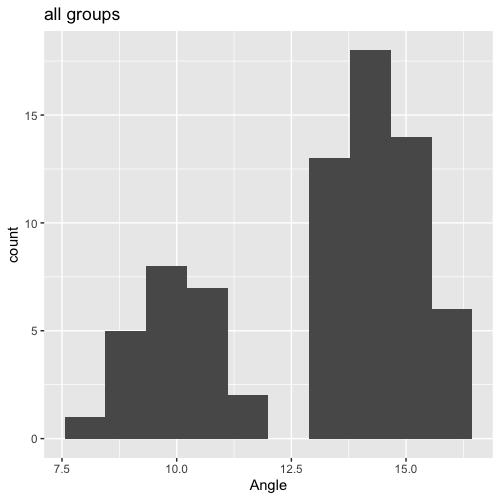
\includegraphics[width=1.5in]{1_all_a_hist.png}
	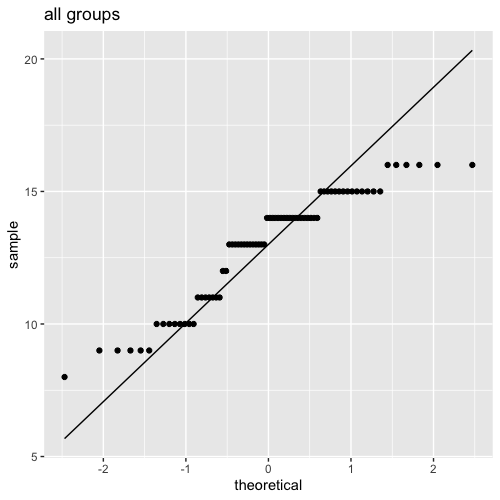
\includegraphics[width=1.5in]{1_all_a_qq.png}
	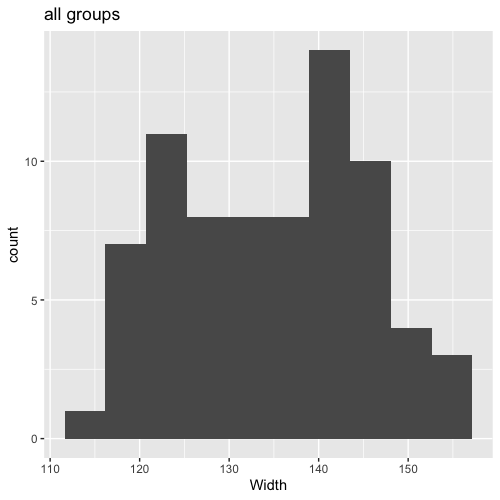
\includegraphics[width=1.5in]{1_all_w_hist.png}
	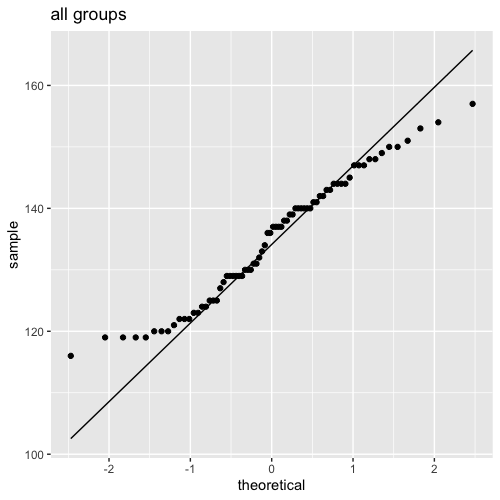
\includegraphics[width=1.5in]{1_all_w_qq.png}
\end{center}
\begin{center}
	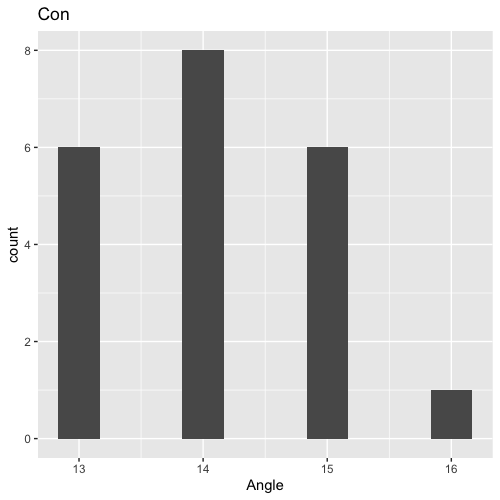
\includegraphics[width=1.5in]{1_Con_a_hist.png}
	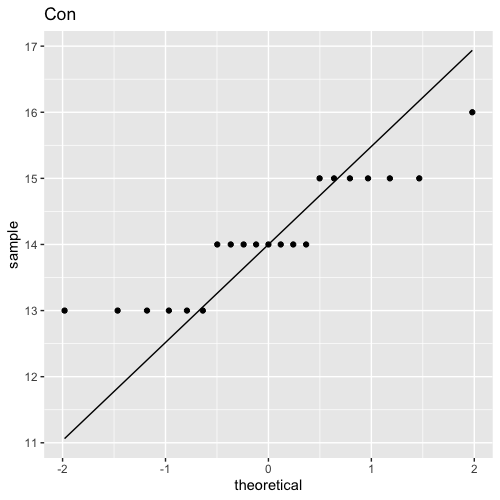
\includegraphics[width=1.5in]{1_Con_a_qq.png}
	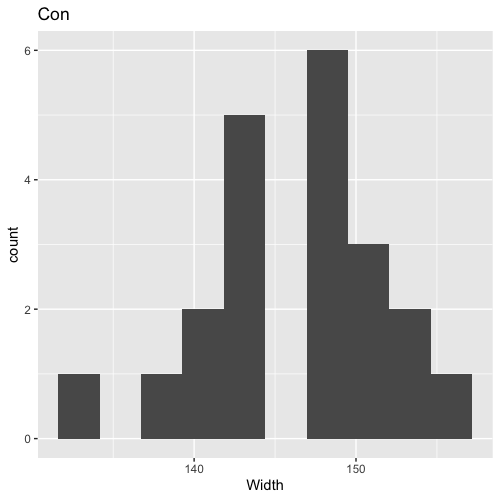
\includegraphics[width=1.5in]{1_Con_w_hist.png}
	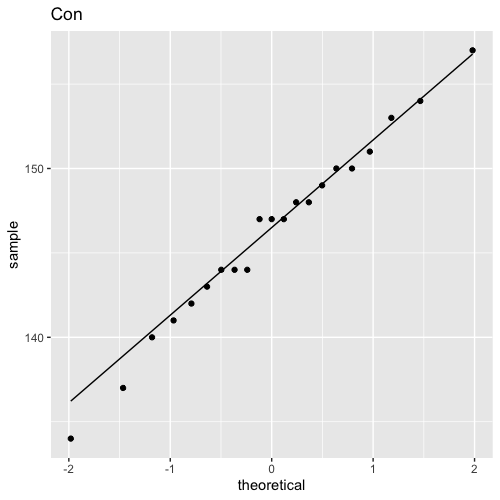
\includegraphics[width=1.5in]{1_Con_w_qq.png}
\end{center}
\begin{center}
	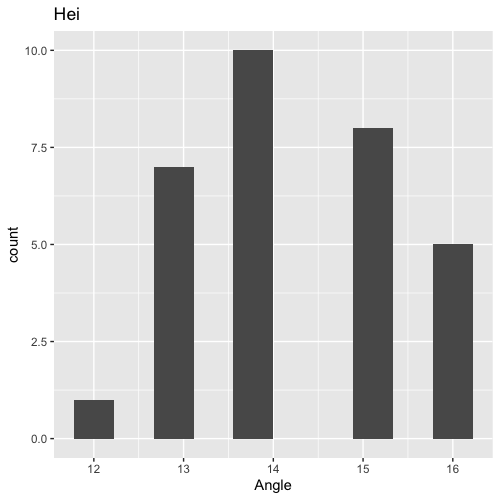
\includegraphics[width=1.5in]{1_Hei_a_hist.png}
	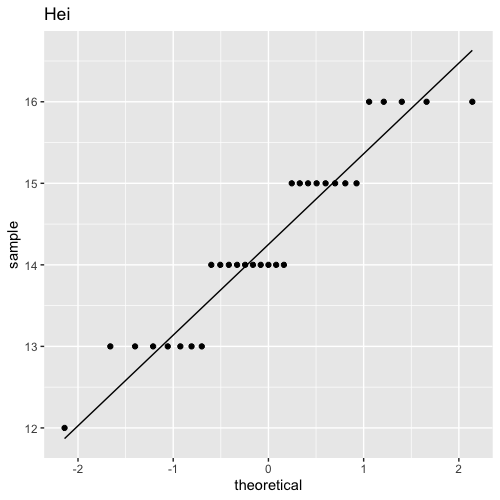
\includegraphics[width=1.5in]{1_Hei_a_qq.png}
	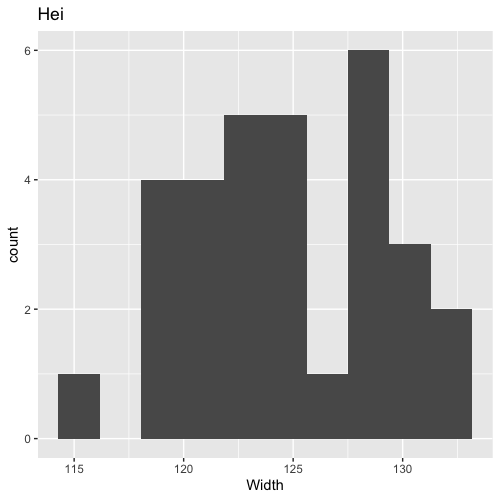
\includegraphics[width=1.5in]{1_Hei_w_hist.png}
	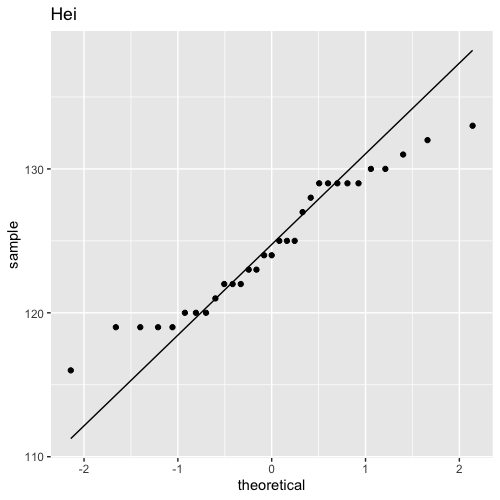
\includegraphics[width=1.5in]{1_Hei_w_qq.png}
\end{center}
\begin{center}
	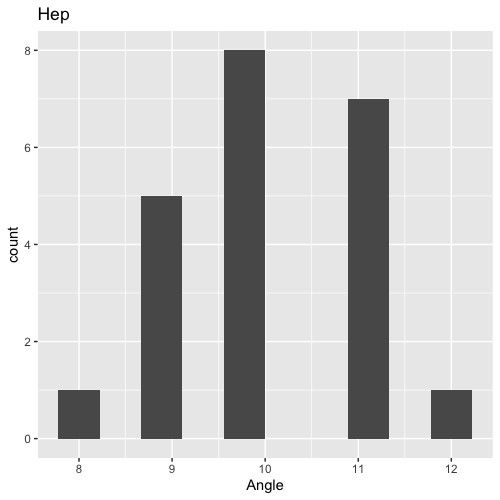
\includegraphics[width=1.5in]{1_Hep_a_hist.png}
	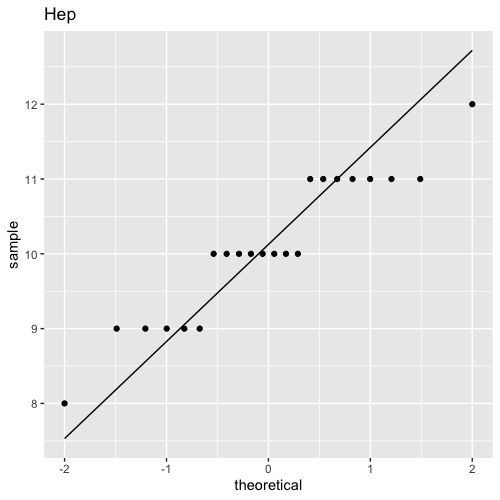
\includegraphics[width=1.5in]{1_Hep_a_qq.png}
	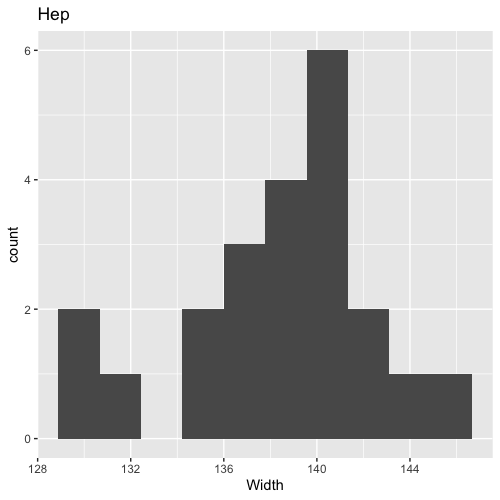
\includegraphics[width=1.5in]{1_Hep_w_hist.png}
	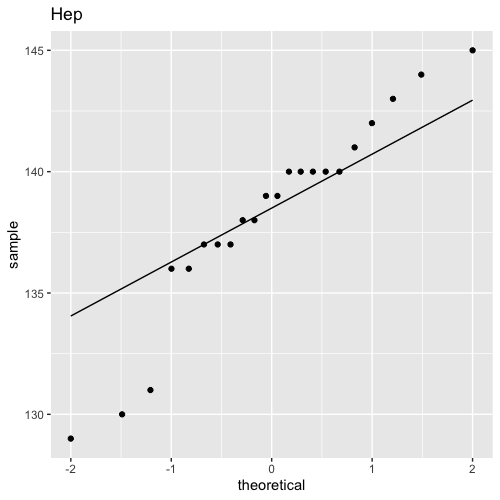
\includegraphics[width=1.5in]{1_Hep_w_qq.png}
\end{center}

	The histogram of all species reveals a bimodal distribution for both dependent variables. The separation into multiple groups is due to the distribution by species, made evident by the scatterplot matrix shown below. For both Angle and Width, there is an apparent overlap of the distributions of two of the three beetle species in the right mode of the distribution of all observations. This finding about the density and location of observations helps to explain the findings in the QQ plot, which shows `light' left tails and `heavy' right tails in both distributions. The histograms for each individual species reveal a central tendency to the distributions, but do not conclusively suggest that the data are distributed normally. Shapiro-Wilks and PPCC tests are formed on the null hypothesis that the data are normally distributed, and many of these tests fail given reasonable confidence levels, $\alpha$. However, it should be noted that the sample counts for each of the three species fall below $30$, which are relatively small and may explain the departure from normality.

\begin{center}
	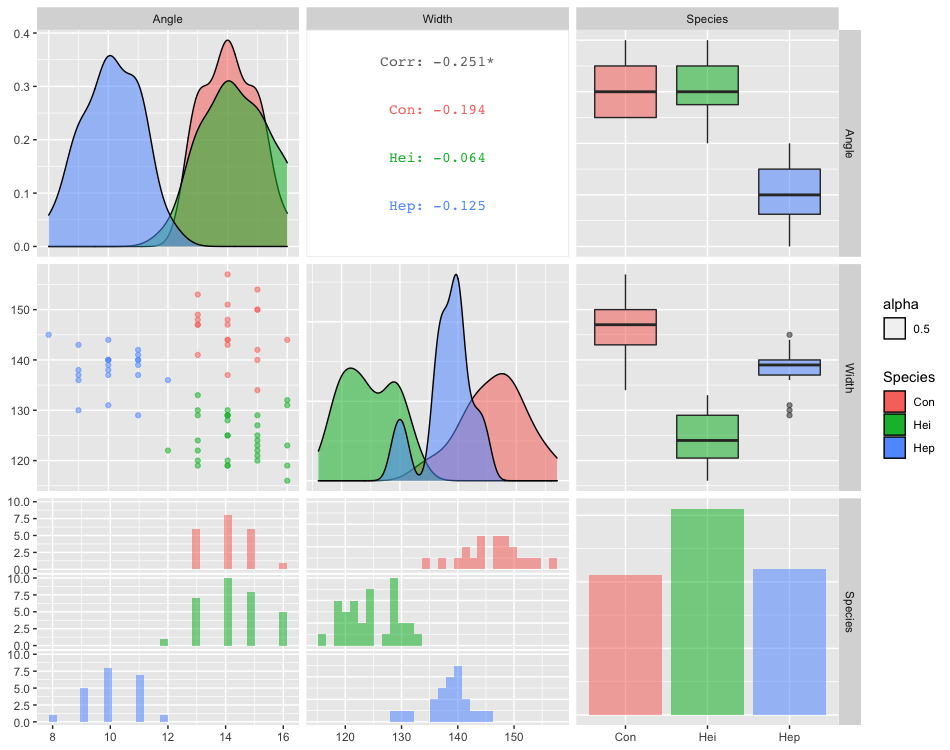
\includegraphics[width=3.0in]{1_scattermatrix.png}
	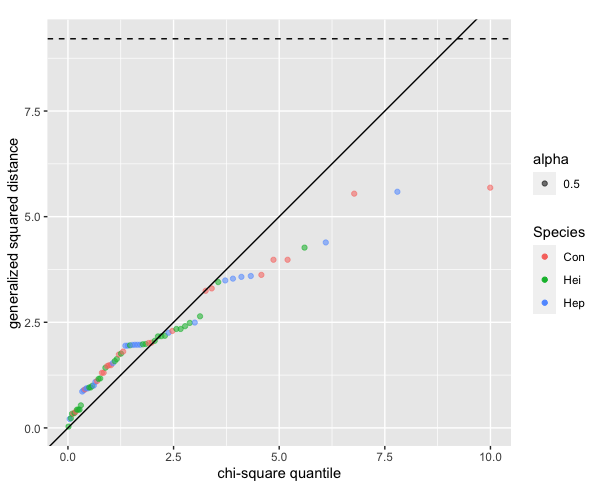
\includegraphics[width=3.0in]{1_chisq.png}
\end{center}

\begin{center}
\begin{tabular}{| c | c c | c c | c c |} 
	\hline
	transformed & group & variable & Shapiro-Wilks & p-value & correlation test & p-value \\
	\hline
	&&&&&&\\
	no & all & Angle & 0.908 & 5e-05 & 0.956 & 2e-04 \\
	yes & all & Angle & 0.930 & 5e-05 & 0.968 & 2e-04 \\
	&&&&&&\\
	no & all & Width & 0.966 & 0.004 & 0.986 & 0.09 \\
	yes & all & Width & 0.966 & 0.004 & 0.986 & 0.09 \\
	&&&&&&\\
	no & Con & Angle & 0.866 & 8e-04 & 0.935 & 0.017 \\
	yes & Con & Angle & 0.864 & 7e-04 & 0.933 & 0.013 \\
	&&&&&&\\
	no & Con & Width & 0.988 & 0.99 & 0.993 & 0.963 \\
	yes & Con & Width & 0.988 & 0.99 & 0.993 & 0.966 \\
	&&&&&&\\
	no & Hei & Angle & 0.911 & 0.013 & 0.959 & 0.028 \\
	yes & Hei & Angle & 0.904 & 0.009 & 0.956 & 0.018 \\
	&&&&&&\\
	no & Hei & Width & 0.949 & 0.15 & 0.979 & 0.229 \\
	yes & Hei & Width & 0.949 & 0.15 & 0.979 & 0.227 \\
	&&&&&&\\
	no & Hep & Angle & 0.911 & 0.05 & 0.952 & 0.04 \\
	yes & Hep & Angle & 0.909 & 0.04 & 0.952 & 0.04 \\
	&&&&&&\\
	no & Hep & Width & 0.924 & 0.09 & 0.961 & 0.09 \\
	yes & Hep & Width & 0.924 & 0.09 & 0.9761 & 0.09 \\
	&&&&&&\\
	\hline
\end{tabular}
\end{center}

	Consider again the scatterplot matrix, colored by species. This plot provides insight into the bivariate distribution of the dependent variables and reveals three relatively separate clouds of points, each associated with one of the three beetle species. The clouds of points associated with concinna and heptapotamica beetles appear roughly elliptical, whereas those associated with heikertingeri have two highly dense regions. No major outliers appear present given the scatterplot matrix alone. Further supporting this conclusion, a chi-square plot, shown next to the scatterplot matrix, suggests that there are no points in the bivariate representation with statistical distances from the overall center of the data that exceed a threshold of $\mathcal{X}_{p=2}^{2}(0.99) = 9.210$, the critical value of a chi-square distribution with $2$ degrees of freedom given a confidence level of $\alpha =0.01$. Certainly, no outlying values are to blame for the apparent departure from normality. While not presented in this report, it should also be noted that none of the standardized observations exhibit any gross departure ($\sigma = 3$) from the group centers nor from the overall center, further evidence supporting that none of the observations are outliers

	Because the visual analysis as well as the Shapiro-Wilks and PPCC tests suggest a lack of normal tendency in both of the univariate distributions, it is desirable to seek a transformation may help to represent the distributions in a normal form. A Box-Cox analysis of the bivariate data is performed on all of the observations and the observations separated by species.The overall Box-Cox contour plot suggests that $\lambda_{Angle} = 2.5$ may improve the normality, however, this is in conflict with each of the three species-specific Box-Cox contour plots, each of which suggest completely different transformation vectors, $\vec{\lambda}$. 

\begin{center}
	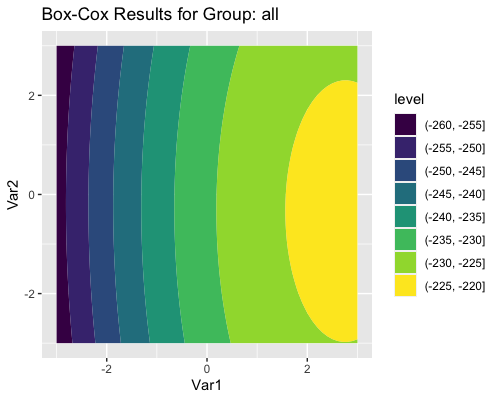
\includegraphics[width=1.5in]{1_bxcx_all.png}
	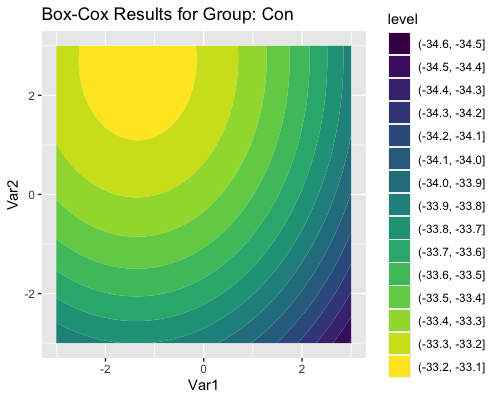
\includegraphics[width=1.5in]{1_bxcx_Con.png}
	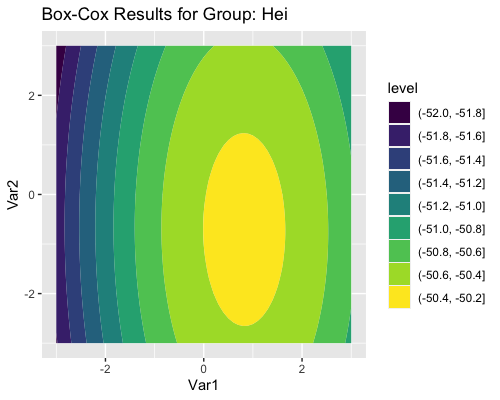
\includegraphics[width=1.5in]{1_bxcx_Hei.png}
	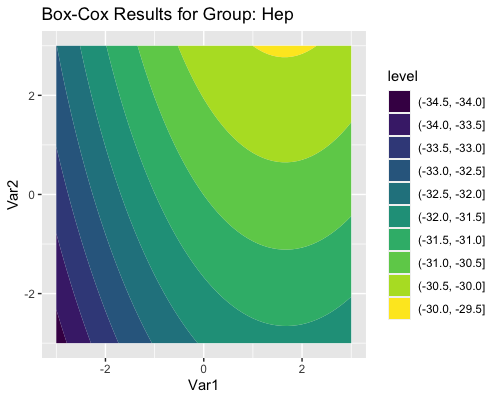
\includegraphics[width=1.5in]{1_bxcx_Hep.png}
\end{center}

	The assumption of normality of the dependent variables is important, but it is still not clear whether a transformation is appropriate yet. It seems reasonable to assume that the measurements are independent of one another (although, sampling methods for beetle selection are not detailed and should be questioned), so the normality of the data may not be as important as the normality of any fitted model residuals. Also, the between species homogeneity of covariance matrices is confirmed via Bartlett, Box-M, and Levene tests on the original data, but these tests fail or nearly fail after transforming the data using $\vec{\lambda}^{\intercal} = \m{2.5 & 1}$ assuming a confidence level of $\alpha = 0.05$. The table below presents the test results for each of the homogeneity of variance tests.

\begin{center}
	\begin{tabular}{| c | c  c  c |}
	\hline
	test & transformed & statistic & p-value \\
	\hline
	&&&\\
	Bartlett & no & 1.717 & 0.423 \\
	& yes & 10.20 & 0.006 \\
	&&&\\
	Box-M & no & 3.288 & 0.771 \\
	& yes & 12.08 & 0.060 \\
	&&&\\
	Levene & no & 0.871 & 0.422 \\
	& yes & 3.756 &  0.028 \\
	&&&\\
	\hline
\end{tabular}
\end{center}

	While there are questions as to the normality of the dependent variables, it appears to be a worse trade-off to transform the data. The underlying assumption of normality should be kept in mind as the analysis proceeds, but this assumption may be mitigated if model residuals are normally distributed in the multivariate analysis of variance (MANOVA) case. The departure from normality is likely due in large part to the small sample sizes previously mentioned.

\begin{enumerate}

\newpage
\item[\bf{(a-b)}]

	A multivariate analysis of variance (MANOVA) is performed on the beetle data. Recall that the independent variable is the Species of beetle. The three different species can be thought of as different `treatments' on an overall average beetle. In the MANOVA model, presented below, the treatments are represented as the $\tau_l,\ l=1,\ 2,\ 3$ \cite[301]{AMSA}. In effect, the MANOVA model seeks to identify if any of the pairs of treatment vectors significantly differ from one another. 

	$$\mf{X}_{lj} = \vec{\mu} + \vec{\tau}_l + \vec{e}_{lj},\ j=1,\ 2,\ \ldots,\ n_l,\ l = 1,\ 2, \ldots,\ g$$

	Interpretted in context, a MANOVA model will reveal whether any two species of beetles significantly differs in either Angle, Width, or Angle and Width. Analogous to the univariate analysis of variance (ANOVA), a MANOVA table provides a simple overview of the decomposition of the variance exhibited by the data. However, instead of sum of squares (variance), the sum of squares and cross products (variance-covariance) are presented as matrices. 

\begin{center}
\begin{tabular}{| c c c |} 
	\hline
	Source of Variation & Matrix SSCP & degrees of freedom \\
	\hline
	&&\\
	Treatment & $\mf{B} = \m{262.97&-366.46\\-366.46&6186.65}$ & $2$ \\
	&&\\
	Residual & $\mf{W} = \m{72.01&-39.73\\-39.73&1634.69}$ & $71$ \\
	&&\\
	\hline
	&&\\
	Total (corrected) & $\mf{T} = \m{334.98&-406.18\\-406.18&7821.35}$ & $73$ \\
	&&\\
	\hline
\end{tabular}
\end{center}

	The statistic formed from the MANOVA table is based on the likelihood ratio statistic called Wilk's Lambda, $\mf{\Lambda}$. A variety of tests can be obtained using this statistic, all of which are used to test the hypothesis set:

	$$H_0:\ \vec{\mu}_i = \vec{\mu}_j,\ H_a:\ \vec{\mu}_i \neq \vec{\mu}_j,\ some\ i \neq j$$

	Which is equivalent to testing the equality of the treatment means, $\tau_i = \tau_j$. The most commonly used statistic used for MANOVA is Wilk's test. Given $p=2$ and $g=3$, the exact distribution of this test is defined as:

	$$\frac{n_1+n_2+n_3-g-1}{g-1} \cdot \frac{1-\sqrt{\mf{\Lambda^*}}}{\sqrt{\mf{\Lambda^*}}} \distras{} F_{2 \cdot (g-1),\ 2 \cdot (n_1+n_2+n_3-g)},\ \mf{\Lambda}^* = \frac{\md{\mf{W}}}{\md{\mf{W} + \mf{B}}}\ \cite[303]{AMSA}$$

	The statistic is calculated in R as $F_{obs} = 125.91$, which greatly exceeds the critical value of the $F$ distribution with the appropriate degrees of freedom and confidence level of $\alpha=0.05$, $2.436$. Therefore, there is sufficient evidence given the sample data to reject the null hypothesis in favor of the alternative. That is, at least one species differs from another in Angle, Width, or Angle and Width. 

	In order for these results to be sound, the underlying assumptions of the MANOVA model need to be satisfied. First, the independent variables should be factors with discrete levels and the dependent variables should be continuous. Observations in the data should be independent of one another, normally distributed, and not contain any univariate or multivariate outliers. Lastly, each of the species' covariance matrices should be homogeneous. As previously established, all but the normality assumption of the dependent variables has been established. While this is still problematic, note that the distribution of the MANOVA model residuals appears to be independent and identically distributed as bivariate normal, as shown in the plot below. This supports the adequacy of the dependent variables explanation of beetle species.

\begin{center}
	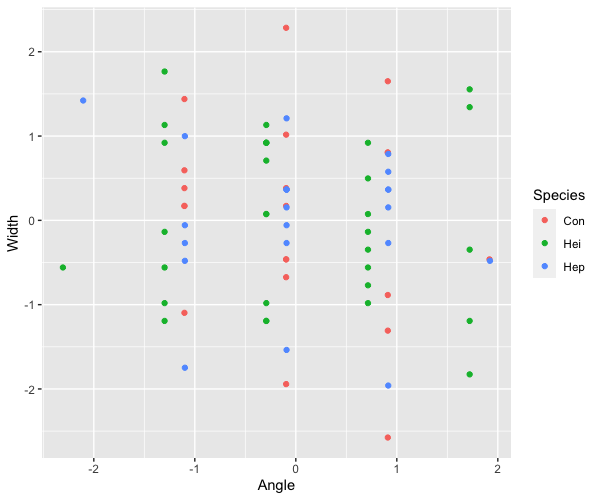
\includegraphics[width=3.0in]{1_b_residuals.png}
\end{center}

\newpage
\item[\bf{(c-d)}]
	Although the MANOVA results suggest at least one pair of the mean vectors of beetle species differ from one another, it gives no indication as to what pair (or pairs) is (are) significantly different. For this case, let us consider the difference between the species concinna and heikertingeri. The hypothesis set under consideration is thus: 

	$$H_0:\ \vec{\mu}_1 = \vec{\mu}_2,\ H_a:\ \vec{\mu}_1 \neq \vec{\mu}_2$$

	Where $\vec{\mu}_1^{\intercal} = \m{14.095 & 146.19}$ represents average Angle and Width for the species concinna and $\vec{\mu}_2^{\intercal} = \m{14.290 & 124.64}$ represents species heikertingeri.	A $95\%$ confidence region for the difference between the two mean vectors defines the test. The statistic for the test is Hotelling's $T^2$ statistic, and the sample version supposing homogeneous covariance matrices is defined below.

	$$\m{\bar{X}_1 - \bar{X}_2}^{\intercal} \m{\p{\frac{1}{n_1} + \frac{1}{n_2}} \mf{S}_{pooled}} \m{\bar{X}_1 - \bar{X}_2} \distras{} \frac{2 \cdot \p{n_1+n_2-2}}{n_1+n_2-p-1} \cdot F_{p,\ n_1+n+2-p-1}\ \cite[285]{AMSA}$$

	The test statistic is calculated in R as $229.1$, which greatly exceeds $6.503$, the critical value of the reference $F$ distribution given a confidence level of $\alpha = 0.05$ ($3.186$) and adjusted by the coefficient displayed in the RHS of the above defined equation ($2.040$). That is, given the sample data, there is sufficient evidence to reject the null hypothesis in favor of the alternative. This means that beetles of the species concinna differ from those of heikertingeri in either Angle, Width, or Angle and Width. Again, as in the MANOVA, the set of assumptions about the different species must be observed. These assumptions do not vary from the MANOVA test. Although excluded from this report, the tests for homogeneity of covariance between these two species was reperformed and the results sustained.

	In order to identify which of the components of these two mean vectors differ from one another, simultaneous confidence intervals and/or Bonferroni confidence intervals can be obtained. First, note that the region defining Hotelling's $T^2$ test when $p=2$ is a two dimensional ellipse, centered at $\bar{X}_1 - \bar{X}_2$, whose axes are determined by the eigenvectors ($\vec{e}_i$) of $S_{pooled}$ with unit length and scaled by the square root of the respective eigenvalue ($\lambda_i$) multiplied by the adjusted critical value of the test ($3.186 \cdot 2.040 =6.503$). The decision rule is to reject $H_0$ if the hypothesized difference vector is not included in the ellipse. The eigenvectors and scaling factors are thus:

	$$\vec{e}_1 = \m{-0.023\\0.999},\ \sqrt{\lambda_1 \cdot \p{\frac{1}{n_1}+\frac{1}{n_2}} \cdot 6.503} = \sqrt{25.5 \cdot 0.079 \cdot 6.503} = 3.638$$
	$$\vec{e}_2 = \m{-0.999\\-0.023},\ \sqrt{\lambda_2 \cdot \p{\frac{1}{n_1}+\frac{1}{n_2}} \cdot 6.503} = \sqrt{1.029 \cdot 0.079 \cdot 6.503} = 0.736$$

	Similarly, the simultaneous confidence intervals are found by projecting the `shadow' of the confidence region onto the axes of each of the variables. If the hypothesized component-wise difference is not contained in the interval, $H_0$ should be rejected. The simultaneous confidence region is a more conservative approach (wider interval) that takes into consideration the covariance between mean vector components, whereas the Bonferroni confidence interval (narrower interval) assumes no covariance between components. The visualization of the confidence region, simultaneous confidence intervals, and Bonferroni confidence intervals is shown in the plot below. 

\begin{center}
	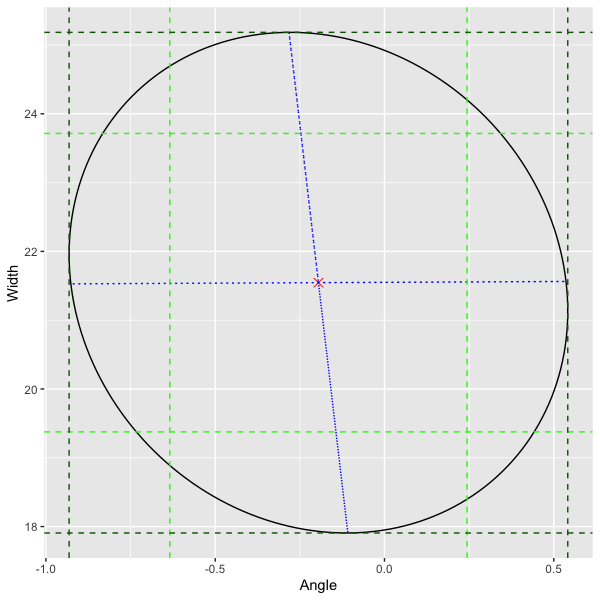
\includegraphics[height=2.5in]{1_d_ellipse.png}
	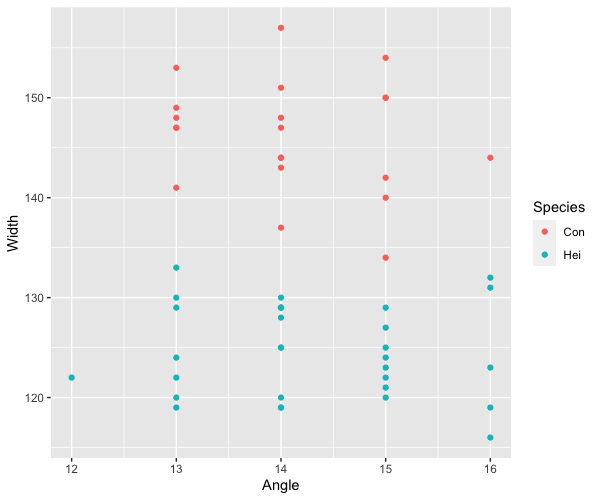
\includegraphics[height=2.5in]{1_d_scatter.png}
\end{center}

	From the confidence ellipse, we see that there is no significant difference in Angle between the two species (the $0$ of angle is included in the simultaneous confidence interval) and that there is a significant difference in Width. Examining a scatterplot of the reduced data and coloring the observations by species, it is clear that the two species are clearly separated on the Width scale but take similar values on the Angle scale, which provide some context to the findings from the confidence region.

\newpage
\item[\bf{(e)}]
	Given the previous findings in this investigation, it is clear that there is separability between the different beetle species. While the relationship between concinna and heptapotamica and the relationship between heikertingeri and heptopotamica were not investigated, the scatterplot matrix showed three visually distinguishable regions between all three species. This suggests that obtaining a classification rule for the species should be possible. Several classification and clustering techniques are next applied to the dataset. Additionally, several validation techniques are used to measure the effectiveness of the classification and clustering methods, ultimately leading to an estimated error rate for the various techniques.

	As established during the MANOVA, homogeneity of the species' covariance matrices is a reasonable assumption given the data. This suggests that a linear discriminant will be suitable for separating and classifying the data. Three discriminant scores for each observation are obtained, utilizing the sample mean for each species. The score based on sample statistics is defined as:

	$$\hat{d_i}(\vec{x}) = \bar{X}_i^{\intercal} S_{pooled}^{-1} \vec{x} - \frac{1}{2} \bar{X}_i^{\intercal} S_{pooled}^{-1} \bar{X}_i + ln(p_i)\ \cite[Lecture~25]{lecture}$$

	Where $p_i$ represents the prior probability of the $i$th species. In this analysis, we take all costs of misclassification to be equal and assume equal prior probabilities for each species. Then, the classification rule is simply to classify $\vec{x}$ to the species with the maximum linear discriminant score. A scatter plot of the data, colored by the known species (below, left). The three regions that define the linear discriminant are plotted in the background. From this plot, it is clear that one observation belonging to species concinna will be classified to heikertingeri.

	Although the assumption of equal covariance matrices is supported, it is worth considering an alternative discriminant score. This quadratic score differs from the linear score by utilizing each species' sample covariance matrix rather than a pooled matrix. Similarly, the scores are generated for each of the three species for each observation. The rule is the same, assign the observation to the species with the largest discriminant score. The quadratic score is defined as:

	$$\hat{d_i}^Q(\vec{x}) = -\frac{1}{2} \md{S_i} -\frac{1}{2} \cdot \p{\vec{x} - \bar{X}_i}^{\intercal} S_i^{-1} \p{\vec{x} - \bar{X}_i} + ln(p_i)\ \cite[Lecture~25]{lecture}$$

	As before, this assumes equal costs for all misclassifications. Another scatterplot is generated, now with the quadratic discrimination regions as the background (below, right). Although the regions now allow some curvature, there is no difference in the classification of the observations.

\begin{center}
	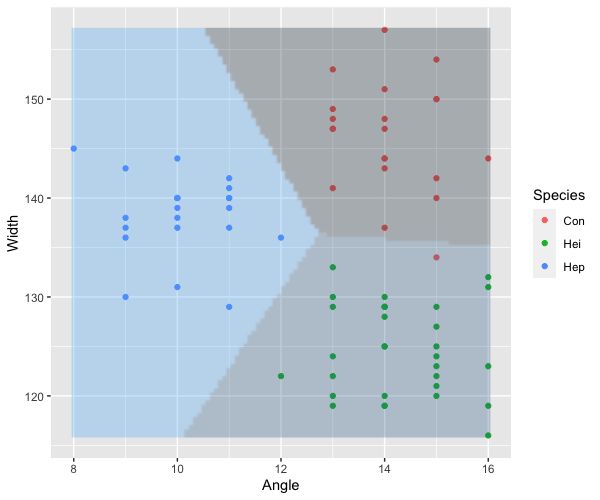
\includegraphics[width=3.0in]{1_e_linear.png}
	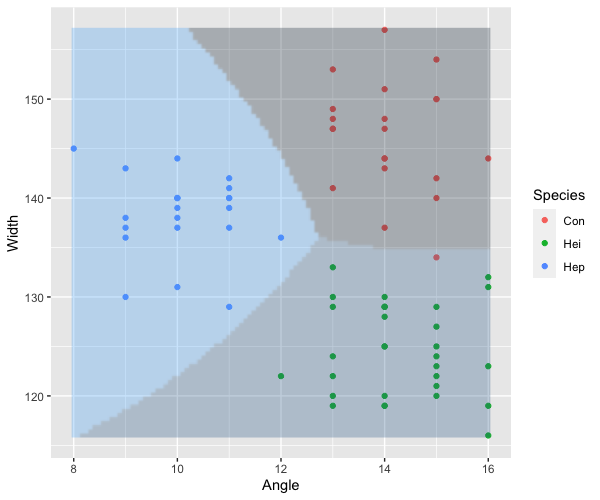
\includegraphics[width=3.0in]{1_e_quadratic.png}
\end{center}

	A simple measure of the apparent error rate (APER) of the classification is obtained by organizing the data into a confusion matrix. In this particular case, the linear and quadratic confusion matrices are identical and are presented below. The diagonals of the matrix represent counts of appropriately classified observations. Then, to obtain a measure of APER, simply sum the off-diagonal entries of the matrix and divide by the total number of classification attempts (observations). For the simple linear and quadratic methods employed, an APER of $\frac{1}{74}=0.135$ is observed.

\begin{center}
\begin{tabular}{| c | c | c c c |}
	\hline
	&& & predicted & \\
	\hline
	&& Con & Hei & Hep \\
	\hline
	& Con& 20 & 1 & 0 \\
	actual & Hei & 0 & 31 & 0 \\
	& Hep & 0 & 0 & 22 \\
	\hline
\end{tabular}
\end{center}

	The classification methods used so far have utilized all of the data to obtain the necessary sample covariance matrices and sample mean vectors needed to obtain the discriminant scores, and hence, the APER obtained by these methods is overly optimistic. More robust methods of validation should be explored in order to better estimate the actual error rate (AER) of classificationof these species of beetles in general. 

	One such method that is relatively easy to implement is $k$ cross-fold validation. In this technique, the data is randomly divided into $k$ groups. One group is reserved and the sample mean vectors and covariance matrices are obtained for each species from the remaining `training' data. The discriminant rules are then applied to the data that was withheld from training. This method can be applied many times to obtain an average APER. When $k=n_1+n_2+n_3$, the techniqueis identical to Lachenbruch's `holdout' method and is also referred to as `one holdout at a time'. When applied to this data, we find no change in the APER for either discriminant scoring method.

	However, for small $k$, there is more variability in the outcome in the classification procedure. Then, if the procedure is replicated a number of times and the average APER calculated for, say, $k=5$, a more realistic estimate of the AER can be obtained. Notice that the linear discriminant seems to provide consistent classification outcomes with any number of folds, but the quadratic rule diminishes slightly when tested with a small number of folds. Altogether, for simplicity and performance, the linear classification should be preferred.

\begin{center}
\begin{tabular}{| c | c c c |}
	\hline
	method & folds (k) & replications & APER \\
	\hline
	&&&\\
	linear discriminant & - & - & 0.01351 \\
	& 74 & - & 0.01351 \\
	& 10 & 100 & 0.01356 \\
	& 5 & 100 & 0.01349 \\
	& 2 & 100 & 0.01347 \\
	&&&\\
	quadratic discriminant & - & - & 0.01351 \\
	& 74 & - & 0.01351 \\
	& 10 & 100 & 0.01609 \\
	& 5 & 100 & 0.01611 \\
	& 2 & 100 & 0.01611 \\
	&&&\\
	k-nearest neighbors (random) & 5 & 10 & 0.1556 \\
	(priors) & 5 & 50 & 0.01644 \\
	&&&\\
	EM clustering (random) & 5 & 10 & 0.1792 \\
	(priors) & 5 & 50 & 0.01516 \\
	&&&\\
	\hline
\end{tabular}
\end{center}

	The classification methods used so far have required knowledge of the true classes of the training data and hence are a form of supervised learning. Within class information allowed the algorithms to take advantage of good initial conditions (priors) for assigning observations to classes. It is interesting then to compare these methods to an unsupervised method requiring no such prior knowledge. 
	
	Two clustering methods, $k$ nearest neighbors and expectation-maximization (EM), provide such a comparison. For each method, a random version of the method is implemented that randomly seeds mean vectors for the three classes and a non-random version is implemented that uses training sample mean vectors for initial conditions. For the EM method,$2$ by $2$ identity matrices are used for the initial covariance matrix estimates. Notice that the random version of the method performs with a higher APER, but still offers good performance overall. The non-random versions of the method are comparable to the discriminant classification methods used.

\end{enumerate}

\newpage
\begin{thebibliography}{}

\bibitem{car}
Fox, John and Sanford Weisberg (2019). 
\textit{An R Companion to Applied Regression, Third Edition}. 
Thousand Oaks CA: Sage. https://socialsciences.mcmaster.ca/jfox/Books/Companion/

\bibitem{heplots}
Fox, John, Michael Friendly and Georges Monette (2020). 
\textit{heplots: Visualizing Tests in Multivariate Linear Models}. 
R package version 1.3-7. URL https://CRAN.R-project.org/package=heplots

\bibitem{AMSA}
Johnson, Richard and Dean Wichern (2007).
\textit{Applied Multivariate Statistical Analysis}.
Sixth Edition. Pearson Prentice Hall, New Jersey.

\bibitem{rstatix}
Kassambara, Alboukadel (2020). 
\textit{rstatix: Pipe-Friendly Framework for Basic Statistical Tests}. 
R package version 0.6.0. https://CRAN.R-project.org/package=rstatix

\bibitem{caret}
Kuhn, Max (2020). 
\textit{caret: Classification and Regression Training}. 
R package version 6.0-86. https://CRAN.R-project.org/package=caret

\bibitem{lecture}
Li, Fang (2020).
\textit{Lecture Notes from STAT 52400: Applied Multivariate Analysis}.

\bibitem{ppcc}
Pohlert, Thorsten (2020). 
\textit{ppcc: Probability Plot Correlation Coefficient Test}.
R package version 1.2. https://CRAN.R-project.org/package=ppcc

\bibitem{GGally}
Schloerke, Barrett, Di Cook, Joseph Larmarange, Francois Briatte, Moritz Marbach, Edwin Thoen, Amos Elberg and Jason Crowley (2020). 
\textit{GGally: Extension to 'ggplot2'}. 
R package version 2.0.0. https://CRAN.R-project.org/package=GGally

\bibitem{MASS}
Venables, W. N. and Ripley, B. D. (2002). 
\textit{Modern Applied Statistics with S}.
Fourth Edition. Springer, New York. ISBN 0-387-95457-0

\bibitem{tidyverse} 
Wickham, Hadley et al., (2019).
\textit{Welcome to the tidyverse}. 
Journal of Open Source Software, 4(43), 1686, https://doi.org/10.21105/joss.01686

\end{thebibliography}
\end{document}
